\section{Lezione 22}%
\label{sub:Lezione 22}
\subsection{Mixing delle traiettorie}%
\label{sub:Mixing delle traiettorie}
Se abbiamo delle divergenze esponenziali nelle traiettorie dello spazio delle fasi allora possiamo dedurre che il sistema realizzi un mixing.\\
Si parla di mixing quando la misura di due traiettorie distinte ha la proprieta:
\[
    \left<A(t)B(t)\right> \to  \left<A\right>\left<B\right> \qquad \text{con } t\to \infty
.\] 
Vediamo cosa significa in pratica a partire da un famoso esempio:
\begin{exmp}[Gatto di Arnold]
    Il sistema del gatto di Arnold è descritto dalla seguente mappa:
    \[
        T: \quad
	\begin{pmatrix} x_{n+1} \\ y_{n+1} \end{pmatrix}  = 
	\begin{pmatrix} 
	    1 & 1 \\
	    1 & 2
	\end{pmatrix} 
	\begin{pmatrix} x_n \\ y_n \end{pmatrix} 
	\quad \text{mod}x = \text{mod}y = 1
    .\]
    La mappa è Hamiltoniana poiché ha determinante unitario. \\
    Per capire come questo sistema realizza il mixing andiamo a studiare i punti fissi. Sappiamo che un punto fisso deve finire in se stesso dalla applicazione della mappa:
    \[
        \begin{cases}
            x = x+y -n \\
	    y = x + 2y - m
        \end{cases}
    .\] 
    In cui $n \in \left[0,1\right]$, $m \in \left[0,2\right]$ per via del modulo unitario.\\
    In particolare si ha $n=1$ solo se la $x$ esce dal quadrato unitario, lo stesso vale per la $y$ che potrebbe aver bisogno anche di una spinta di $-2$ per rientrare.\\
    Risolvendo per i punti fissi otteniamo i seguenti valori:
    \[
        y = n \qquad x = - y + m
    .\] 
    Quindi i punti fissi sono i quattro vertici del quadrato che, in sostanza, sono tutti lo stesso punto per via del modulo unitario.\\
    La mappa tangente invece è equivalente alla mappa stessa (si ottiene con le derivate miste):
    \[
        \begin{pmatrix} 
	    1 & 1 \\
	    1 & 2
	\end{pmatrix} 
    .\] 
    Gli autovalori e gli autovettori di questa mappa sono:
    \[
        \lambda_{\pm}= \frac{3 \pm \sqrt{5} }{2} \qquad
	\xi_{\pm} = \begin{pmatrix} 1 \\ \frac{1 \pm \sqrt{5} }{2} \end{pmatrix} 
    .\] 
    Notiamo che essendo la mappa Hamiltoniana i due autovalori devono essere uno l'inverso dell'altro, questa proprietà è rispettata dai $\lambda_{\pm}$.\\
    Possiamo quindi vedere come sono fatte le varietà stabili/instabili attorno ai quattro punti fissi. \\
    Scostandosi da ogni punto fisso di una quantità $\epsilon$ (per ciascuna delle due coordinate) e inserendo il punto "scostato" nella mappa si ottengono i seguenti risultati:
    \[\begin{aligned}
	&(\epsilon,\epsilon)\to (2\epsilon, 3\epsilon)\\
	& (1-\epsilon, \epsilon) \to (1, 1+\epsilon) \to (1, \epsilon)
    .\end{aligned}\]
    Quindi il primo punto è instabile, il secondo è stabile (non sappiamo se ci siamo posti esattamente sul manifold uscente/entrante, sappiamo solo che nei pressi degli scostamenti valutati c'è uno di questi due).\\
    I risultati per gli altri punti sono riportati in figura \ref{fig:21_stab_instab}.
    \begin{figure}[H]
        \centering
        \incfig{21_stab_instab}
	\caption{\scriptsize Stabilità dei punti fissi nel sistema di Arnold.}
        \label{fig:21_stab_instab}
    \end{figure}
    \noindent 
    Visto che abbiamo valutato gli autovalori della mappa tangente possiamo prendere il maggiore e valutarvi l'esponente di Lyapunov:
    \[
	\sigma  = \ln (\lambda_+) = \ln\left(\frac{3 + \sqrt{5} }{2}\right) > 0 
    .\] 
    Il sistema presenta caos.
    Possiamo vedere cosa succede alla mappa iterata due volte, facciamo il prodotto tra le matrici:
    \[
        \begin{pmatrix} 
	    1 & 1 \\
	    1 & 2
	\end{pmatrix} 
        \begin{pmatrix} 
	    1 & 1 \\
	    1 & 2
	\end{pmatrix} 
	= 
	\begin{pmatrix} 
	    2 & 3\\
	    3 & 5
	\end{pmatrix} 
	\qquad \text{mod}1
    .\] 
    Possiamo cercare nuovamente i punti fissi, procedendo nello stesso modo visto nel caso della mappa iterata una sola volta si arriva a ($x, y$):
    \[
        \left(\frac{1}{5}, \frac{3}{5}\right); \ \left(\frac{2}{5}, \frac{1}{5}\right); \ 
	\left(\frac{3}{5}, \frac{4}{5}\right); \ \left(\frac{4}{5}, \frac{2}{5}\right)
    .\] 
    E tutti questi sono ancora punti iperbolici i cui manifold si incrociano formando di nuovo caos. Gli autovalori della mappa tangente questa volta sono:
    \[
        \lambda_{\pm} = \frac{7 \pm \sqrt{45}}{2}
    .\] 
    Quindi abbiamo una mappa che induce una dinamica molto complicata e caotica già dalle prime iterazioni.
\end{exmp}
\noindent
\begin{exmp}[Trasformazione di Baker]
    Riprendiamo la trasformazione di Baker già vista nella precedente lezione:
    \[\begin{aligned}
	&
        \begin{cases}
            x_{n+1} = 2 x_n\\
	    y_{n+1} = y_n /2
	\end{cases} & \quad \text{se } 0 \le x_n \le  1 /2\\
	& 
        \begin{cases}
            x_{n+1} = 2 x_n - 1\\
	    y_{n+1} = y_n /2 + 1 /2
	\end{cases} & \quad \text{se } 1 /2 < x_n \le 1 \\
    \end{aligned}\]
    I punti fissi della mappa sono:
    \[
	(0, 0); \quad (1, 1)
    .\] 
    Andiamo a vedere la mappa linearizzata:
    \[
	M = 
        \begin{pmatrix} 
	    1 & 0 \\
	    0 & 2
	\end{pmatrix} 
    .\] 
    Gli autovalori sono già sulla diagonale, siamo quindi in una base di autovettori:
    \[
        \omega_1 = \begin{pmatrix} 1\\0 \end{pmatrix} \qquad
	\omega_2 = \begin{pmatrix} 0 \\1 \end{pmatrix} 
    .\] 
    Andando a vedere gli scostamenti dai punti fissi si scopre che questi sono iperbolici, rammentiamo che per capirlo è proprio necessario andare a studiare/simulare la dinamica nei pressi del punto fisso.
    \begin{figure}[H]
        \centering
        \incfig{22_baker}
        \caption{\scriptsize Punti iperbolici nel sistema di Baker.}
        \label{fig:22_baker}
    \end{figure}
    \noindent
    Potremmo andare a vedere la mappa iterata due volte, scopriremo che i punti fissi (che diventano 4) sono ancora iperbolici.
    \subsubsection{Bernoulli Shift}%
    \label{subsub:Bernoulli Shift}
    La trasformazione di Beker ha un'altra importante caratteristica, riprendiamo la notazione binaria per rappresentare l'evoluzione dei numeri nella mappa: 
    \[
        x_n = \sum_{J<0}^{} 2^{J}a_J \qquad y_n = \sum_{k>0}^{} 2^{-k} b_k
    .\]
    Se prendiamo come $\vect{x}_0$ iniziale un numero irrazionale (tra $0$ e $1$) si ha che la sequenza di $a_i\ldots, b_j\ldots$ è infinita. \\
    Se applichiamo a questo numero una trasformazione di Beker otteniamo un numero completamente random (quando si fa nuovamente il cambio di base da $2$ a $10$). Questa caratteristica del sistema è detta Bernoulli Shift e può essere utilizzata per generare numeri random (a partire da una dinamica del tutto deterministica!). 
\end{exmp}
\noindent
\subsection{Mappe non Hamiltoninane}%
\label{sub:Mappe non Hamiltoninane}
\begin{exmp}[Henon Map]
    Prendiamo l'ennesimo sistema che porta il nome di Henon:
    \[
        \begin{cases}
            x_{n+1} = 1 - a x_n^2 + y_n\\
	    y_{n+1} = bx_n
        \end{cases}
    .\] 
    Nello specifico Henon studiò questa mappa con i parametri: $a = 1.4$, $b = 0.3$.\\
    La mappa tangente può essere ricavata dalle derivate:
    \[
        \begin{pmatrix} \delta x_{n+1}\\ \delta y_{n+1} \end{pmatrix} =
	\begin{pmatrix} 
	    -2ax_n & 1 \\
	    b & 0
	\end{pmatrix} 
	\begin{pmatrix} \delta x_n \\ \delta y_n \end{pmatrix} 
    .\] 
    \[
        M = 
	\begin{pmatrix} 
	    -2ax_n & 1 \\
	    b & 0
	\end{pmatrix} 
    .\] 
    Visto che il determinante di $M$ è diverso da zero abbiamo una mappa non Hamiltoniana. Il determinante ci dice anche come la mappa trasforma lo spazio delle fasi:
    \[
	\text{det}(M) = - b \implies  \left|\text{det}(M)\right| < 1 
    .\] 
    Essendo $b$ minore di 1 in modulo la mappa dovrebbe contrae lo spazio delle fasi $dxdy$. Provando a simulare la mappa invece si ottengono oggetti di questo tipo:
    \begin{figure}[H]
        \centering
	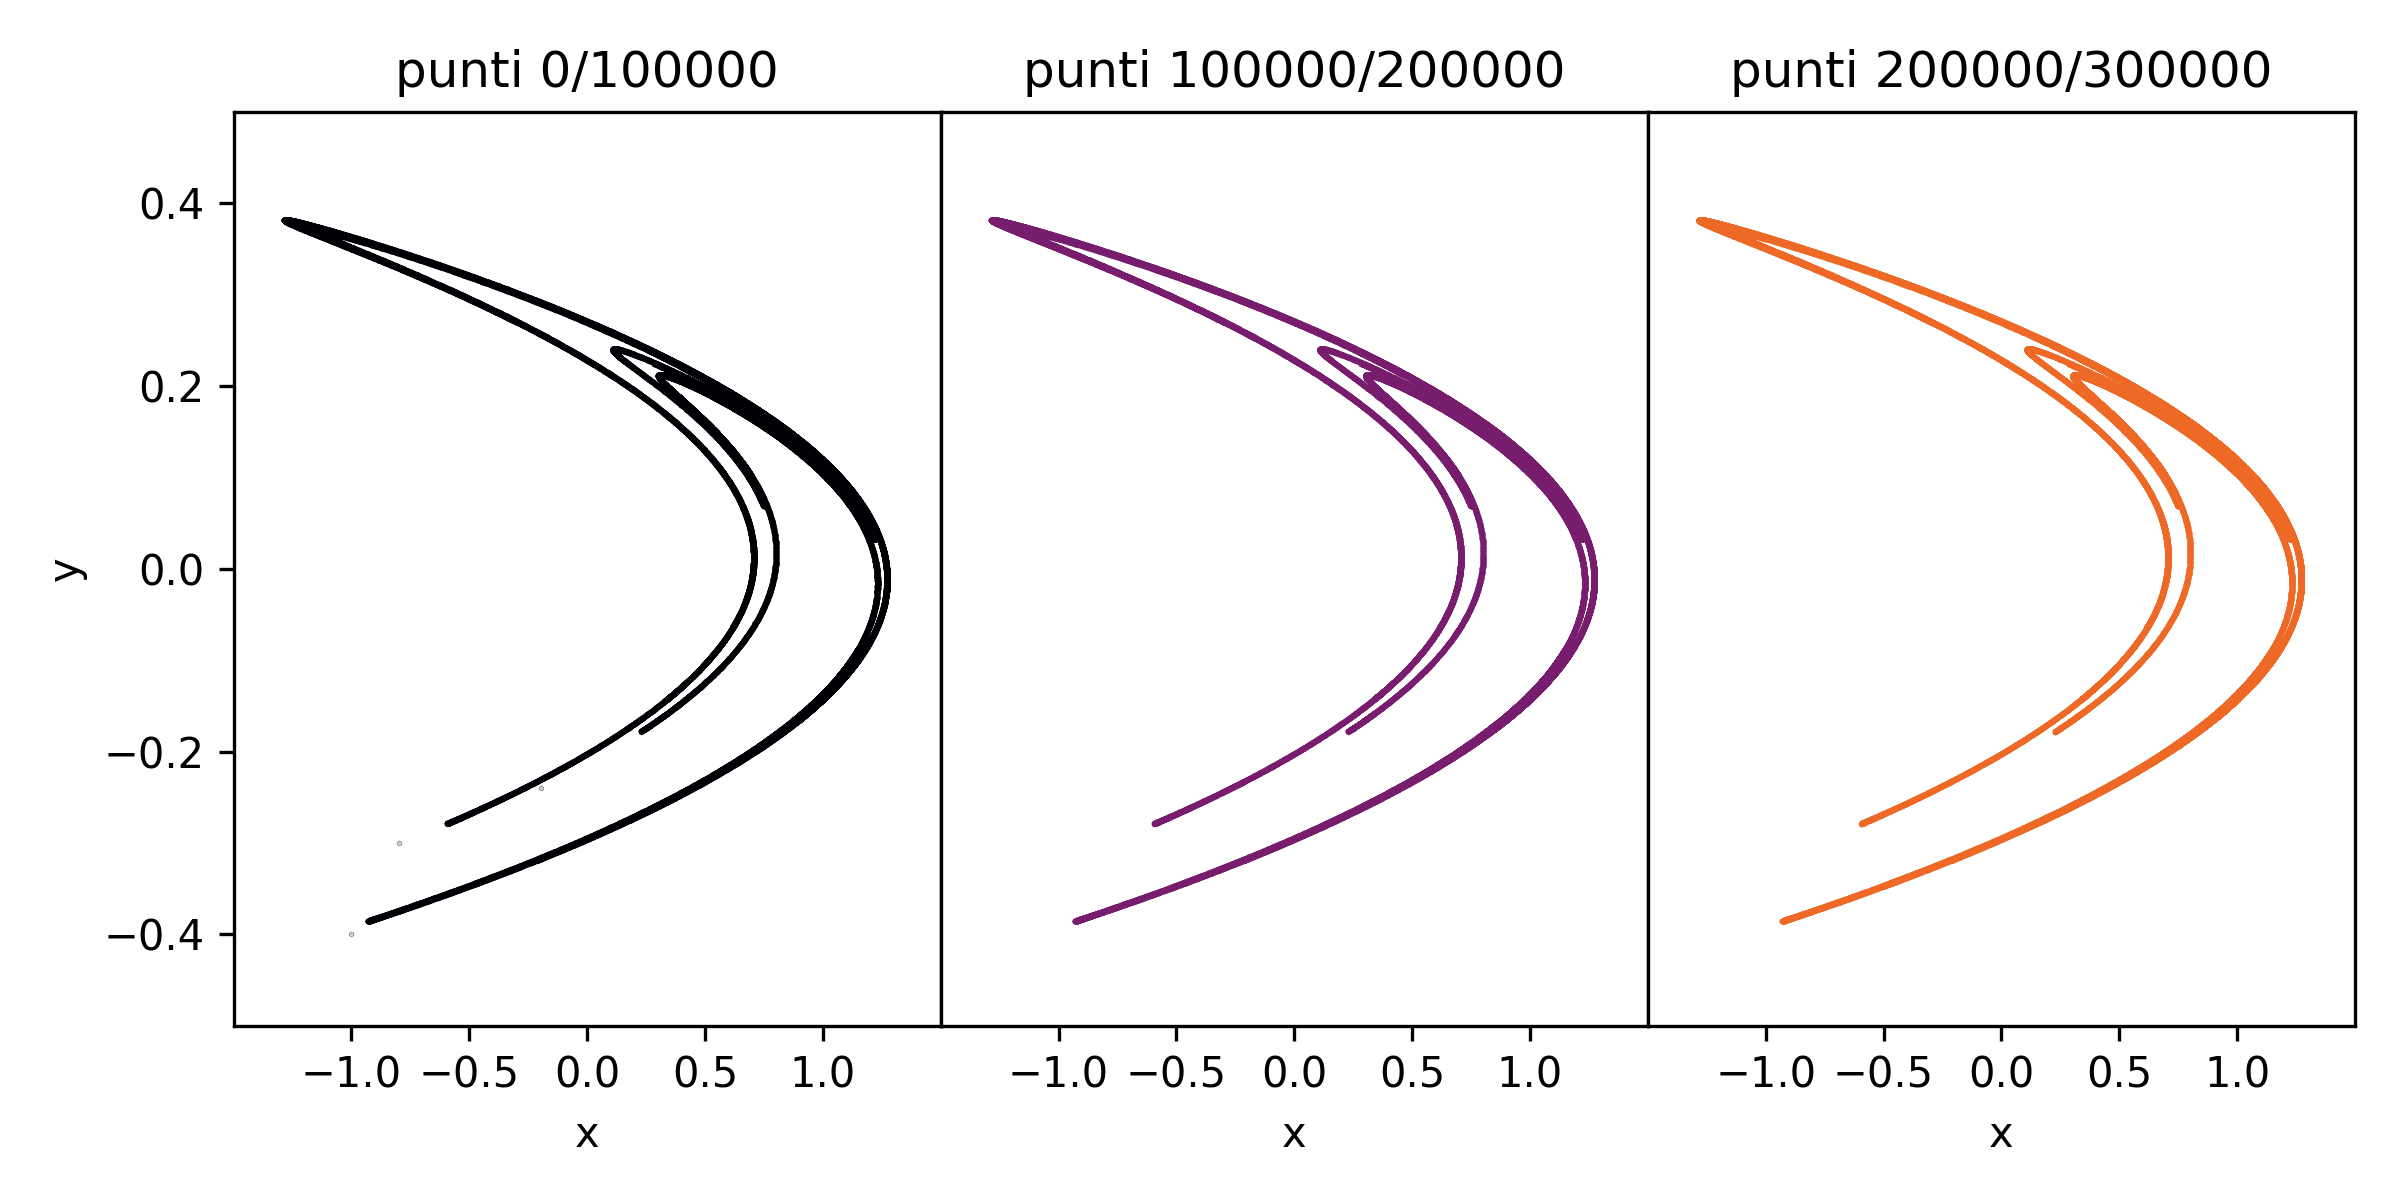
\includegraphics[width=0.45\textwidth]{figures/22_henonmap.png}
	\caption{\scriptsize Mappa di Henon integrata per valori iniziali $(-1, 0.4)$. Si riportano le prime $3\cdot 10^{5}$ iterazioni in 3 blocchi: non cambia nulla dalle prime alle ultime iterazioni. La mappa non doveva contrarre lo spazio delle fasi (che occupa)?}
        \label{fig:figures-22_henonmap-png}
    \end{figure}
\end{exmp}
\noindent
Prima di procedere diamo una importante definizione:
\begin{redbox}{Attrattore}
    Un attrattore è un insieme (set) di punti che attrae la dinamica di un determinato sistema.
\end{redbox}
\noindent
\begin{exmp}[Attrattore di Lorenz]
    Prendiamo la seguente mappa:
    \[
        \begin{cases}
	    \dot{x} = \sigma (y-x)\\
	    \dot{y} = -xz + rx - y \\
	    \dot{z} = xy - bz
        \end{cases}
    .\] 
    I parametri di questo modello sono quantità fisiche, il sistema infatti venne sfruttato per descrivere la fluidodinamica del moto atmosferico da Lorenz. Quest'ultimo voleva dimostrare che nella fluidodinamica atmosferica c'è una forte dipendenza dalle condizioni iniziali.
    \[\begin{aligned}
	&\sigma = \frac{\mu c_p}{k} \\
	&r = \text{num. di Raileigh} \\
	& b = \text{fattore geometrico}
    .\end{aligned}\]
    In cui $\mu$ è la viscosità dell'aria, $c_p$ il suo calore specifico mentre $k$ è la conducibilità. 
    Fisicamente $\sigma$ descrive il meccanismo con cui il sistema può scambiare calore.\\
    Il numero di Rayleigh invece è $>1 (<1)$ se il sistema presenta convezione (conduzione).\\ 
    Per ultimo $b$ è legato al fatto che le ipotesi per questo moto prevedono delle particolari geometrie. \\
    Anche questa mappa assume una forma molto particolare e suggestiva nello spazio delle fasi (Si mostra l'evolvere di una sola condizione iniziale):
    \begin{figure}[H]
        \centering
	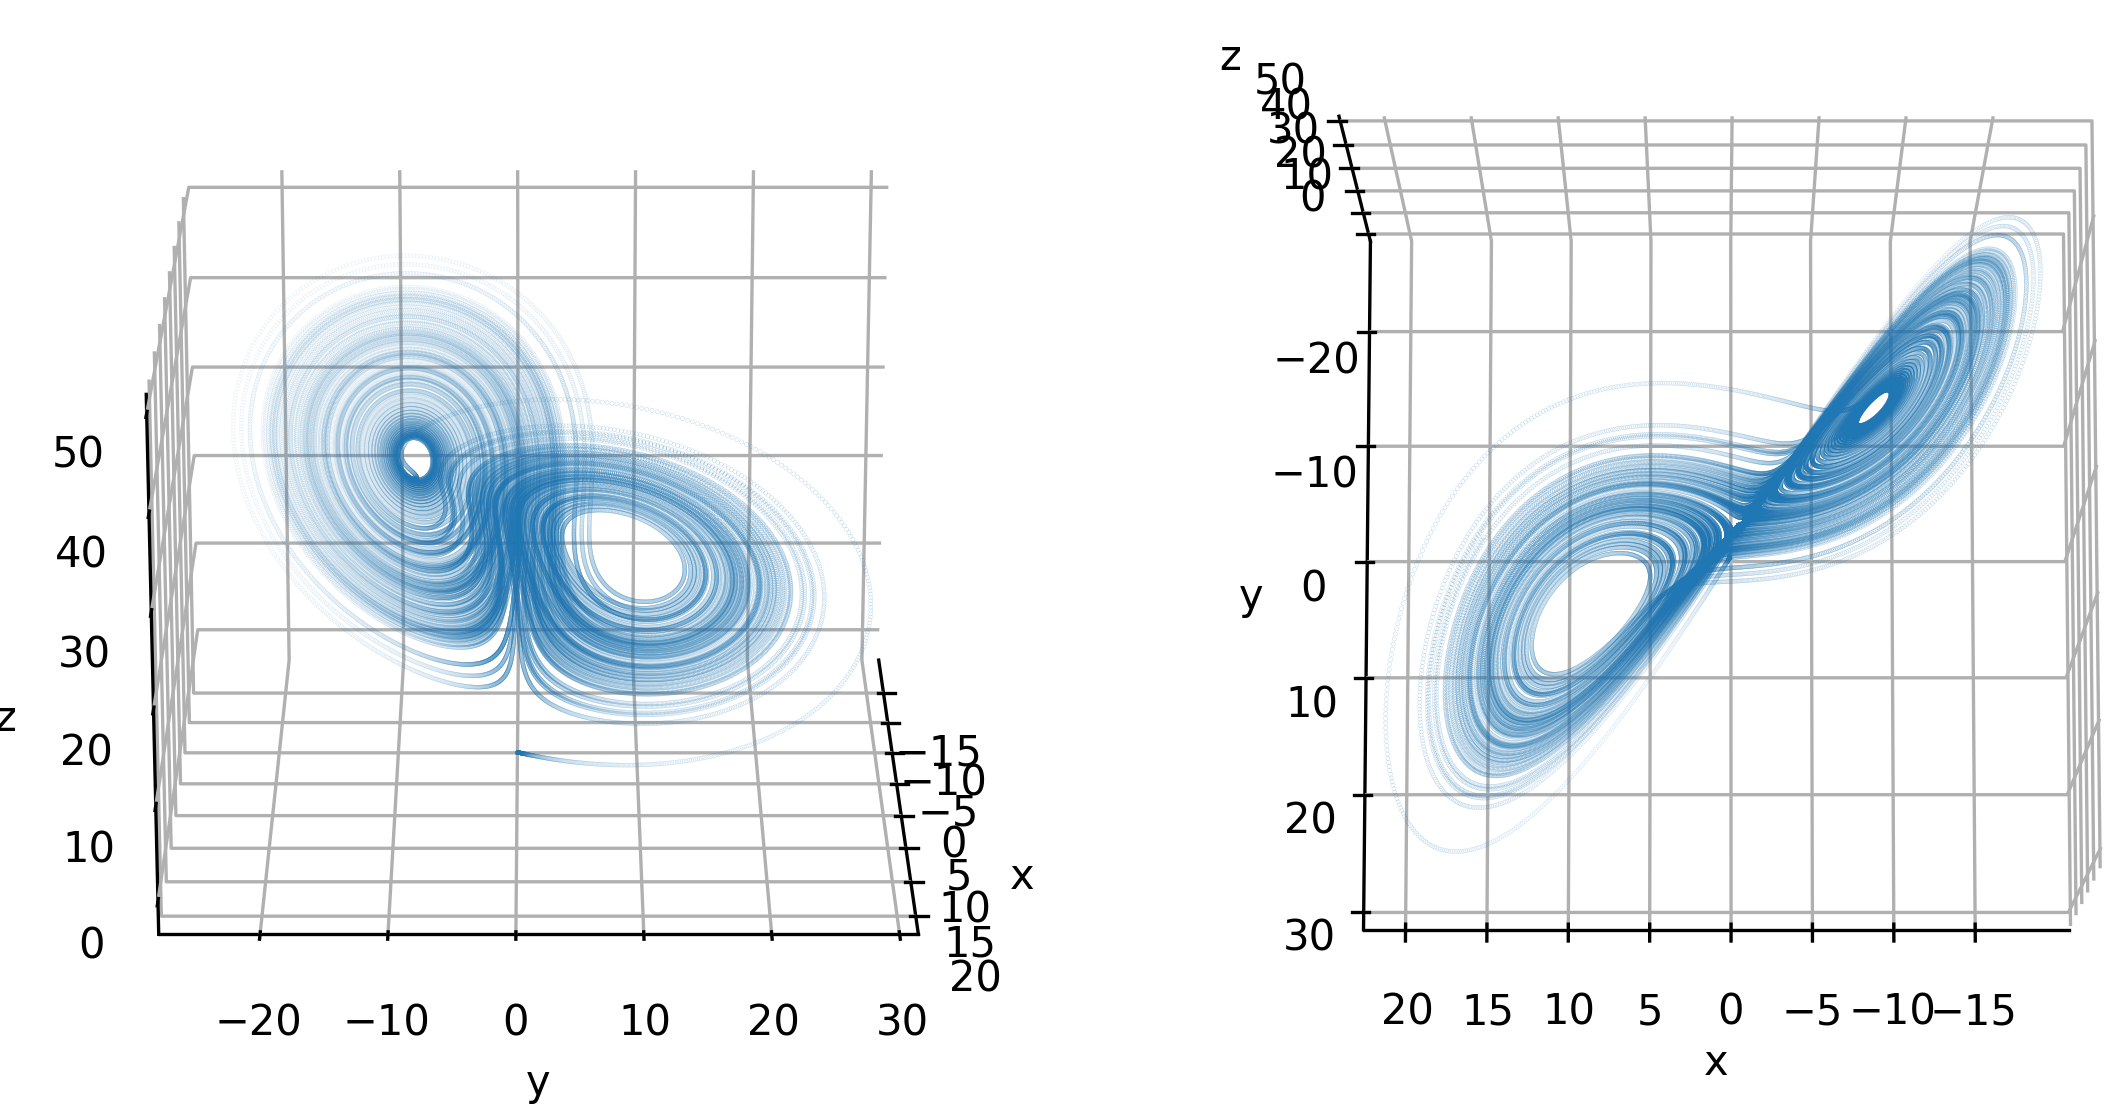
\includegraphics[width=0.45\textwidth]{figures/22_lorenz.png}
        \caption{\scriptsize Attrattore di Lorenz.}
        \label{fig:figures-22_lorenz-png}
    \end{figure}
    Le tre variabili del sistema rappresentano:
    \begin{itemize}
        \item $x$ la convezione del sistema.
	\item $y$ La variazione di temperatura.
	\item La distorsione di $y$ rispetto ad un gradiente lineare di temperatura.
    \end{itemize}
    Quello che fa il modello di Lorenz è descrivere il moto dei fluidi all'interno dei Rolls atmosferici: zone in cui nella parte bassa il fluido è caldo mentre in quella alta il fluido è freddo.\\
    Calcoliamo la "divergenza" della mappa $\nabla \vect{v}$:
    \[
        \nabla \vect{v}  = \frac{\partial }{\partial x} \dot{x} + \frac{\partial }{\partial y} \dot{y} + \frac{\partial }{\partial z} \dot{z} = 
	- (b + \sigma  + 1)
    .\] 
    Quindi visto che $b, \sigma$ sono solitamente maggiori di zero anche questa mappa dovrebbe tendere a collassare nello spazio delle fasi.\\
    Possiamo cercare i punti critici della mappa imponendo che le tre equazioni siano nulle, risolvendo il sistema emergono i seguenti punti:
    \[\begin{aligned}
	& 1)  \ x = y = 0 \\
	& 2) \ y = \pm \sqrt{b (r-1)} \qquad z = r-1 \quad \text{con }r>1
    .\end{aligned}\]
    Possiamo adesso linearizzare le equazioni per valutare la stabilità dei punti fissi, la mappa tangente valutata nel punto $(0, 0, 0)$ ha la struttura:
    \[
        \begin{pmatrix} \delta\dot{x} \\ \delta\dot{y} \\ \delta\dot{z} \end{pmatrix} =
	\begin{pmatrix} 
	    0 & \sigma & -\sigma \\
	    r & -1 & 0\\
	    0 & 0 & -b
	\end{pmatrix} 
	\begin{pmatrix} \delta x\\\delta y\\\delta z \end{pmatrix} 
    .\] 
    Gli autovalori della mappa sono:
    \[\begin{aligned}
	&\lambda_1 = -b\\
	&\lambda_{2, 3} = \frac{-1 \pm \sqrt{1 + 4r\sigma} }{2}
    .\end{aligned}\]
    Il primo autovalore segnala una contrazione poiché $b>0$ quindi $\lambda_1<0$. Per quanto riguarda la coppia $\lambda_{2, 3}$ si ha che sicuramente $\lambda_2$ (quello con il $+$ ) è positivo (se $4r\sigma  > 0$), quindi l'origine potrebbe essere un punto iperbolico.	\\
    Per quanto riguarda il secondo punto fisso invece tralasciamo il conto, il risultato che si ottiene è:
    \[\begin{aligned}
	&\lambda_1 < 0\\
	& \lambda_{2,3} = \alpha\pm i\beta
    .\end{aligned}\]
    Gli autovalori complessi coniugati hanno la particolarità che $\alpha$ cambia di segno per il seguente valore di $r$:
    \[
	\overline{r} = \frac{\sigma  (\sigma  + b + 3)}{\sigma-b-1}
    .\] 
    Quando $\alpha$ assume valori negativi ($r<\overline{r}$) l'oggetto rilassa nel punto fisso, viceversa abbiamo un punto fisso di tipo spirale instabile.
\end{exmp}
\noindent
Il problema che non riusciamo al momento a spiegarci non è il fatto che questi oggetti continuino nel loro moto nello spazio delle fasi, quello che non si riesce a spiegare è il fatto che gli oggetti sembrano continuare a muoversi senza un vincolo. \\
Se pensiamo al pendolo forzato con una forzante periodica abbiamo che la forzante vincolerà il pendolo a fare un moto completamente determinato, quindi di fatto è come se il sistema avesse perso un grado di libertà. \\ 
Con l'attrattore di Lorenz non si riesce a fare il medesimo ragionamento perché il moto sembra continuare a vivere in tutte e tre le dimensioni dello spazio delle fasi.\\
Per spiegare questi fenomeni dobbiamo introdurre dei nuovi concetti: 
\subsection{Il concetto di frattale}%
\label{sub:Il concetto di frattale}
La regola che ne emerge è che data una misura di una quantità $m$ in una determinata scala $l$, una nuova misura $m'$ effettuata con scala $l'$ che sia $N$ volte più piccola di $l$ è legata alla dimensionalità $D$ del sistema nel seguente modo:
\[
    m' = m\cdot N^D 
.\] 
\begin{figure}[H]
    \centering
    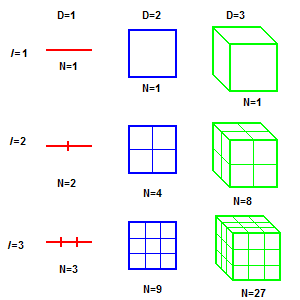
\includegraphics[width=0.3\textwidth]{figures/fractal_wiki.png}
    \caption{\scriptsize Concetto di misura e dimensionalità (wikipedia)}
    \label{fig:figures-fractal_wiki-png}
\end{figure}
\noindent
Quindi il rapporto tra due scale differenti va come:
\[
    \frac{m'}{m} = N^D
.\] 
Chiamando $p$ il rapporto tra le due misure possiamo invertire quest'ultima relazione per ottenere una buona definizione della dimensionalità del sistema $D$:
\begin{redbox}{Dimensione frattale}
\begin{equation}
    D = \frac{\ln p}{\ln N}
    \label{eq:22_dim_fratt}
\end{equation}
\end{redbox}
\noindent
La cosa importante da notare è la generalità della definizione, così generale che appare una cosa controversa: nessuno ci garantisce che $D$ sia intero in quella formula!
\begin{exmp}[Fiocco di Koch]    
Noto questo concetto prendiamo un esempio "pratico". Muniamoci di uno strumento di misura che ha una scala $l$, cerchiamo di adoperarlo per misurare il perimetro di un oggetto che, su questa scala, appare triangolare.
\begin{figure}[H]
    \centering
    \incfig{22_triangolo}
    \caption{\scriptsize triangolo del quale vogliamo misurare il perimetro con la scala più grande.}
    \label{fig:22_triangolo}
\end{figure}
\noindent
Il perimetro misura con questa prima scala $3l$. 
Adesso proviamo a misurarlo con uno strumento avente scala $l /3$, scopriamo che l'oggetto aveva in realtà una forma leggermente diversa:
\begin{figure}[H]
    \centering
    \incfig{22_koch}
    \caption{\scriptsize La struttura si presenta in modo sempre più complicato al rimpicciolire della scala di osservazione.}
    \label{fig:22_koch}
\end{figure}
\noindent
Allora la misura del perimetro diventa (figura \ref{fig:22_koch} a sinistra) $3\cdot 4\cdot l$, diverso dal valore che ci saremmo aspettati per il triangolo "smooth": $3\cdot 3\cdot l$.\\
Iterando ancora il ragionamento la struttura successiva è quella di figura \ref{fig:22_koch} a sinistra: abbiamo un perimetro di $3 \cdot 4\cdot 4 l$.\\
Diventa subito evidente che, se il sistema continua a fare questo scherzetto su tutte le scale, la misura di $D$ per questo esempio ci porta a concludere qualcosa di strano:
\[
    D = \frac{\ln 4}{\ln 3}
.\] 
Otteniamo una dimensionalità che sta a metà tra una superficie ed una linea!\\
Questo sistema è un famosissimo sistema frattale chiamato fiocco di Koch, la struttura "finale" ricorda appunto un fiocco di neve.
\end{exmp}
\noindent
Di insiemi frattali ne esistono tantissimi, solitamente producono tutti effetti grafici mozzafiato ed hanno spesso utilità nel campo dell'"image recognition".\\
Citiamo alcuni esempi di insiemi famosi:
\begin{itemize}
    \item Set di Cantor.
    \item Mandelbrot.
    \item Triangolo di Sierpinski.
    \item Julia.
\end{itemize}
Tornando ai nostri attrattori e le mappe non Hamiltoninane, possiamo definire:
\begin{greenbox}{Attrattore frattale}
    Quando la contrazione di un sistema nello spazio delle fasi incontra strutture sempre più complesse durante la contrazione allora il sistema non si arresta ma continua nel moto.
\end{greenbox}
\noindent
Nei due esempi esaminati sopra (Henon, Lorenz) succede esattamente questo. Questo è il motivo per cui la dinamica non si arresta.
\subsection{Algoritmo di Box Counting per stimare la dimensione frattale}%
\label{sub:Algoritmo di Box Counting per stimare la dimensione frattale}
Prendiamo un esempio che abbiamo già esaminato ma del quale non conosciamo la dimensione frattale: la mappa di Henon. \\
L'idea è quella di suddividere lo spazio delle fasi in quadranti in modo ricorsivo. Per ognuno di questi quadranti si cerca di verificare se sono presenti punti della mappa all'interno.
\begin{figure}[H]
    \centering
    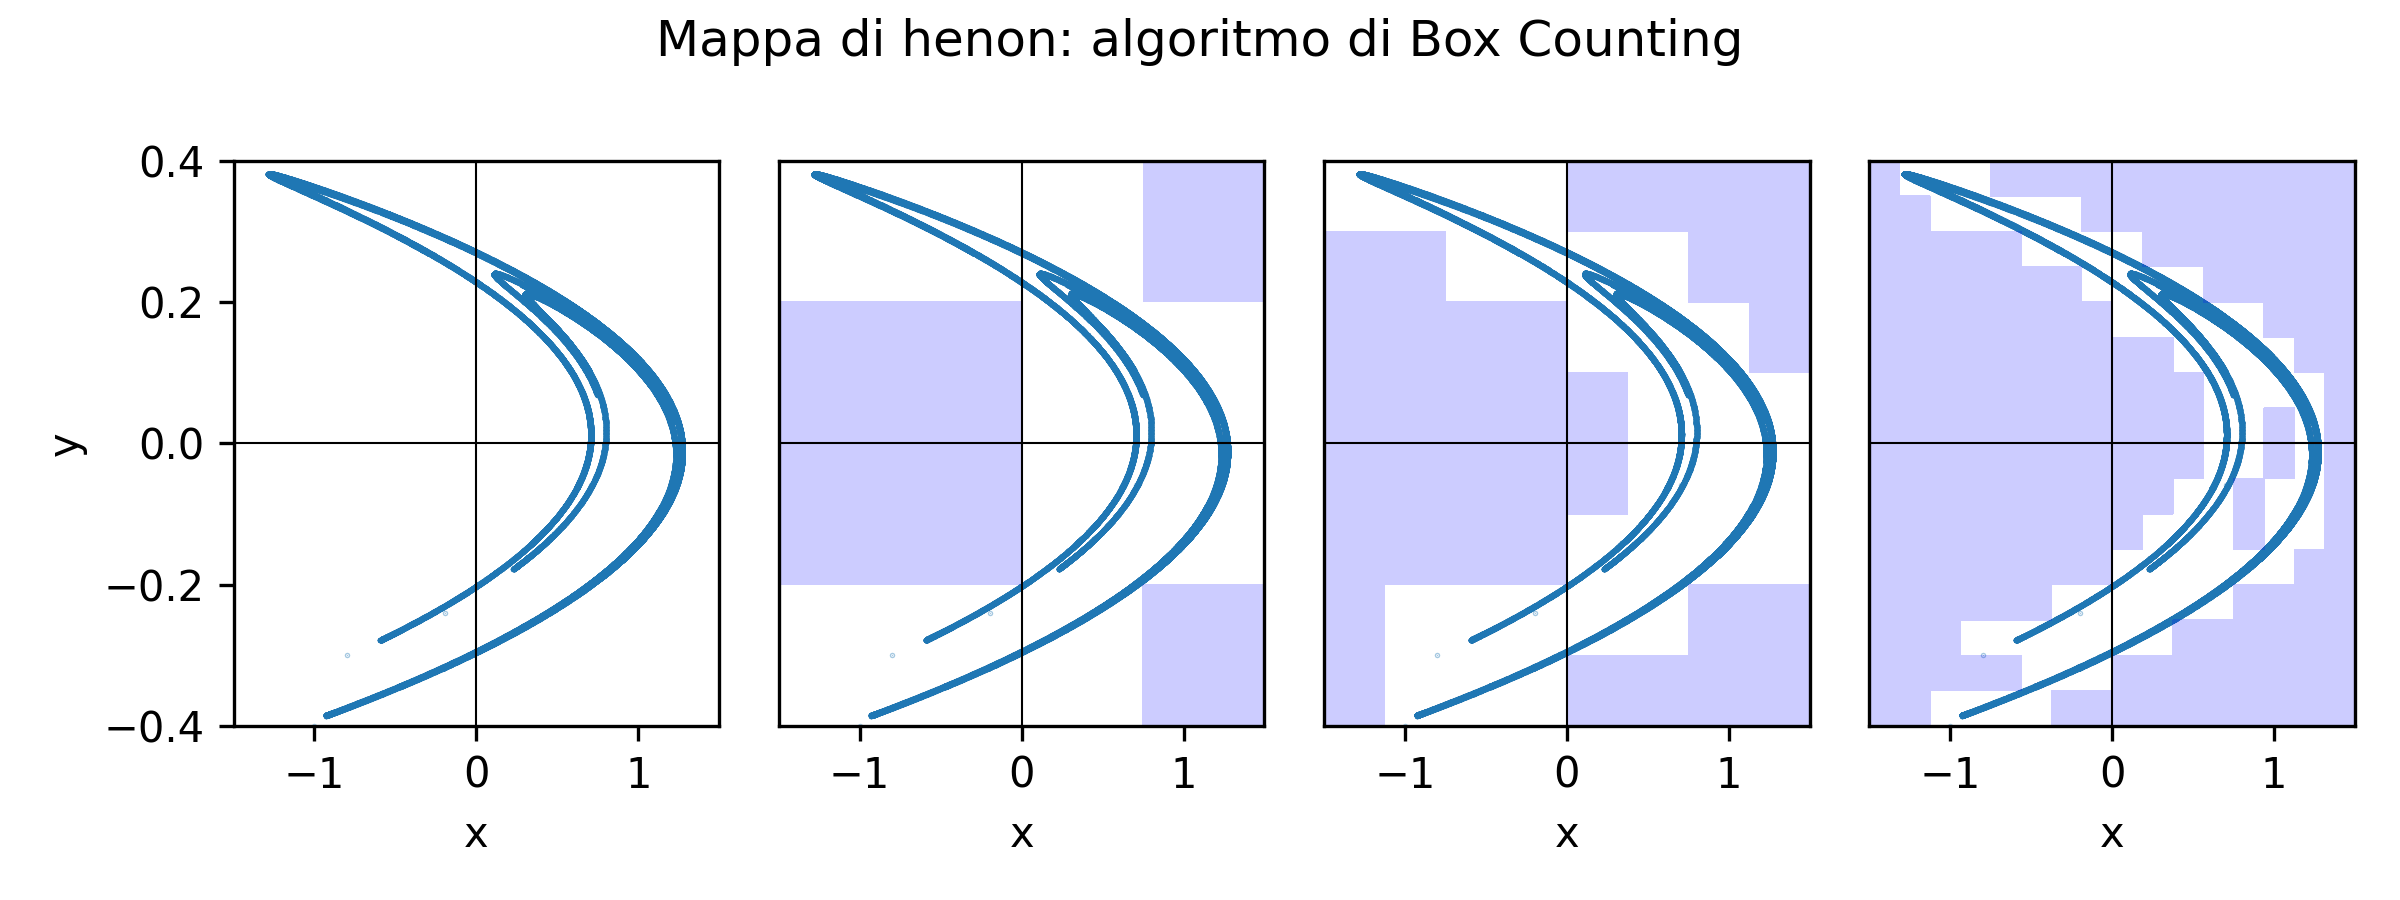
\includegraphics[width=0.45\textwidth]{figures/22_henonmap_box.png}
    \caption{\scriptsize Quadranti sempre più piccoli occupati dai punti della mappa.}
    \label{fig:figures-22_henonmap_box-png}
\end{figure}
\noindent
In conclusione si valuta quanti quadrati sono occupati rispetto alla suddivisione scelta (una potenza di ($1 /2$)).
\begin{itemize}
    \item $1 /2 \to 4$.
    \item $1 /4 \to 10$.
    \item $1 /8 \to 27$.
\end{itemize}
Procedendo in questo modo e continuando a dividere lo spazio in quadrati sempre più piccoli possiamo trovare la dimensione del sistema con la formula \ref{eq:22_dim_fratt}.\\
In questo caso $N$ è proprio il numero che sta al denominatore per l'elenco sopra (2, 4, 8\ldots).\\
Effettuando varie misure di $p$ (il numero di quadrati occupati) al variare di $N$ ed effettuando un fit lineare in $\ln (N), \ln (p)$ si ottiene:
\begin{figure}[H]
    \centering
    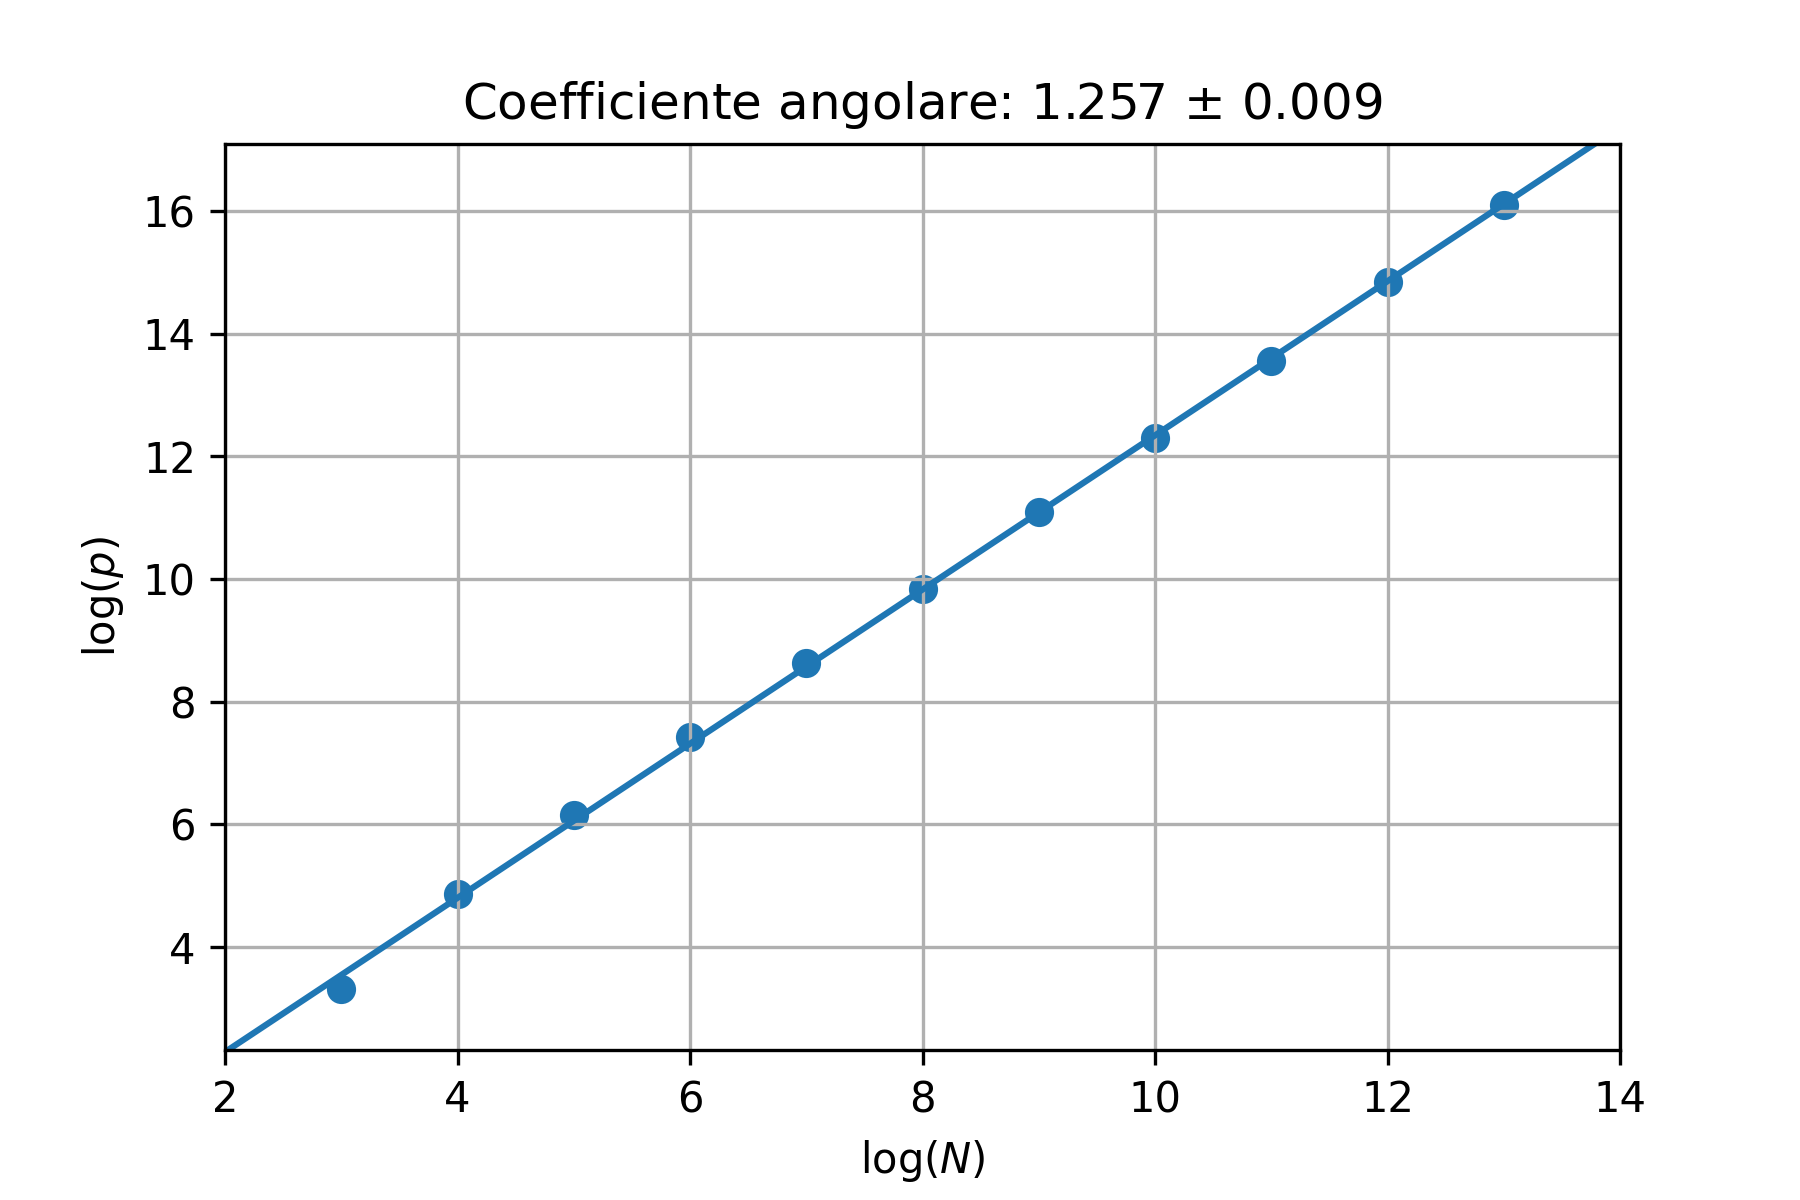
\includegraphics[width=0.5\textwidth]{figures/22_box_fit.png}
    \caption{\scriptsize Fit lineare: la conclusione del metodo di Box counting. \\
    Il coefficiente angolare rappresenta la dimensionalità del sistema ed il logaritmo è in base 2.\\
    I numeri sugli assi non ci permettono di apprezzare il costo computazionale di questa operazione\ldots}
    \label{fig:figures-22_box_fit-png}
\end{figure}
\noindent
Si ottiene una dimensione frattale compatibile con quella scritta da Wikipedia per il sistema: $1.25 \pm 0.02$.\\
Lo stesso metodo può essere applicato all'attrattore di Lorenz, semplicemente in tal caso è necessario usare come scala un cubo (la mappa è 3D).
Nel caso di Lorenz emerge anche un altro problema: la dimensionalità costa computazionalmente. \\
Il metodo di ricerca da me implementato si basa sul metodo della "rubrica telefonica" ed è scritto in python: in due dimensioni inizia già ad accusare (3 secondi per il grafico sopra). Per fare una cosa tridimensionale forse è giusto lasciare il posto a linguaggi più performanti (quando si tratta di loop) come fortran.\\
Consiglio di dare un occhio tra i codici poiché l'algoritmo che ho pensato per implementare la ricerca elude il problema del dover creare una matrice enorme per avere una "buona risoluzione" dello spazio delle fasi\ldots\\
Perché è così importante studiare la dimensione frattale? Perché c'è un teorema che afferma una cosa sconvolgente:
\begin{redbox}{Accenno a teorema Caos-frattale}
    Se un sistema presenta una dimensione frattale non intera allora il sistema è caotico.
\end{redbox}
\noindent
Quindi semplicemente applicando un box counting potremmo dimostrare che il sistema è caotico, senza dover passare dagli altri metodi visti nelle precedenti lezioni.\\
\subsection{Mappa di Henon come meccanismo di Folding e Stretching}%
\label{sub:Mappa di Henon come meccanismo di Folding e Stretching}
La mappa di Henon può esser vista anche come la composizione di 3 mappe distinte, queste tre mappe vengono applicate in successione ad ogni step:
\[
    \begin{cases}
        \overline{x} = x\\
	\overline{y} = y + 1 - a\overline{x}^2
    \end{cases}
\] 
Questa prima mappa trasporta i punti verso una parabola.
\begin{figure}[H]
    \centering
    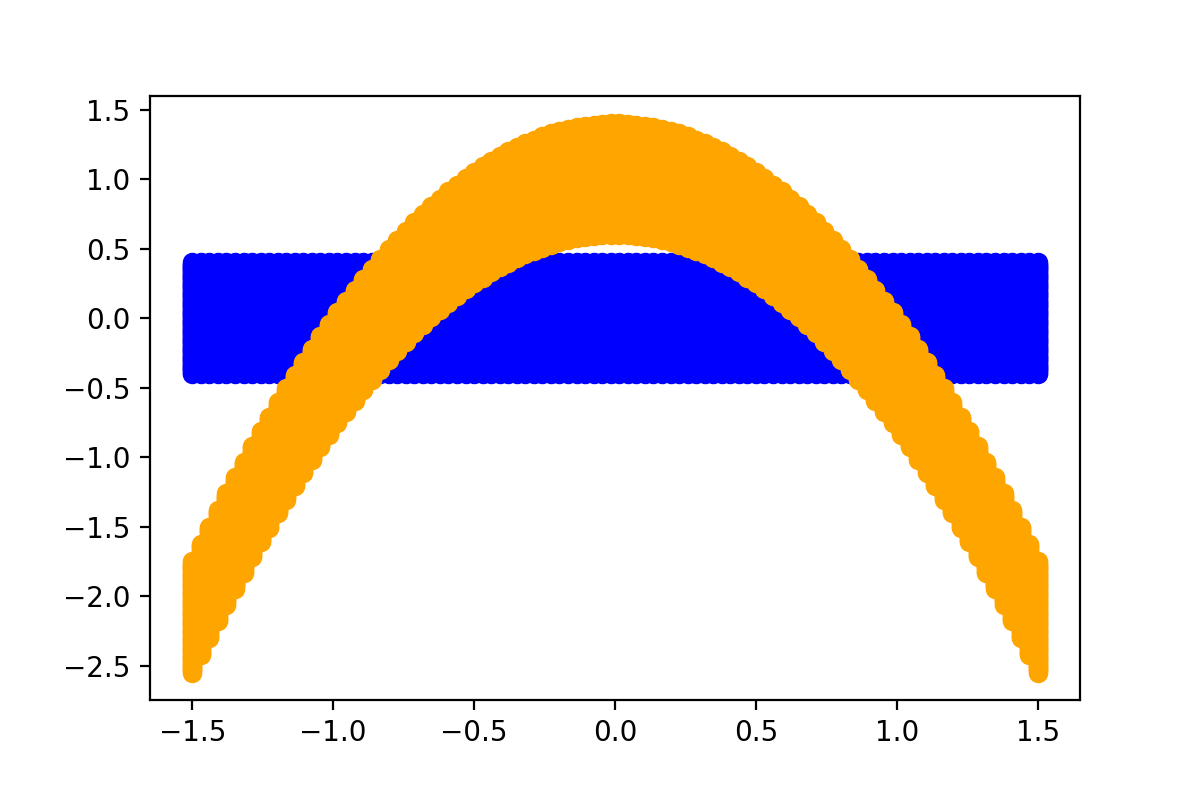
\includegraphics[width=0.3\textwidth]{figures/22_step1henon.png}
    \caption{\scriptsize Prima mappa}
    \label{fig:figures-22_step1henon-png}
\end{figure}
\noindent
La seconda mappa invece comprime i punti sull'asse x:
\[
    \begin{cases}
        \overline{\overline{x}} = b\overline{x}\\
	\overline{\overline{y}} = \overline{y}
    \end{cases}
\] 
\begin{figure}[H]
    \centering
    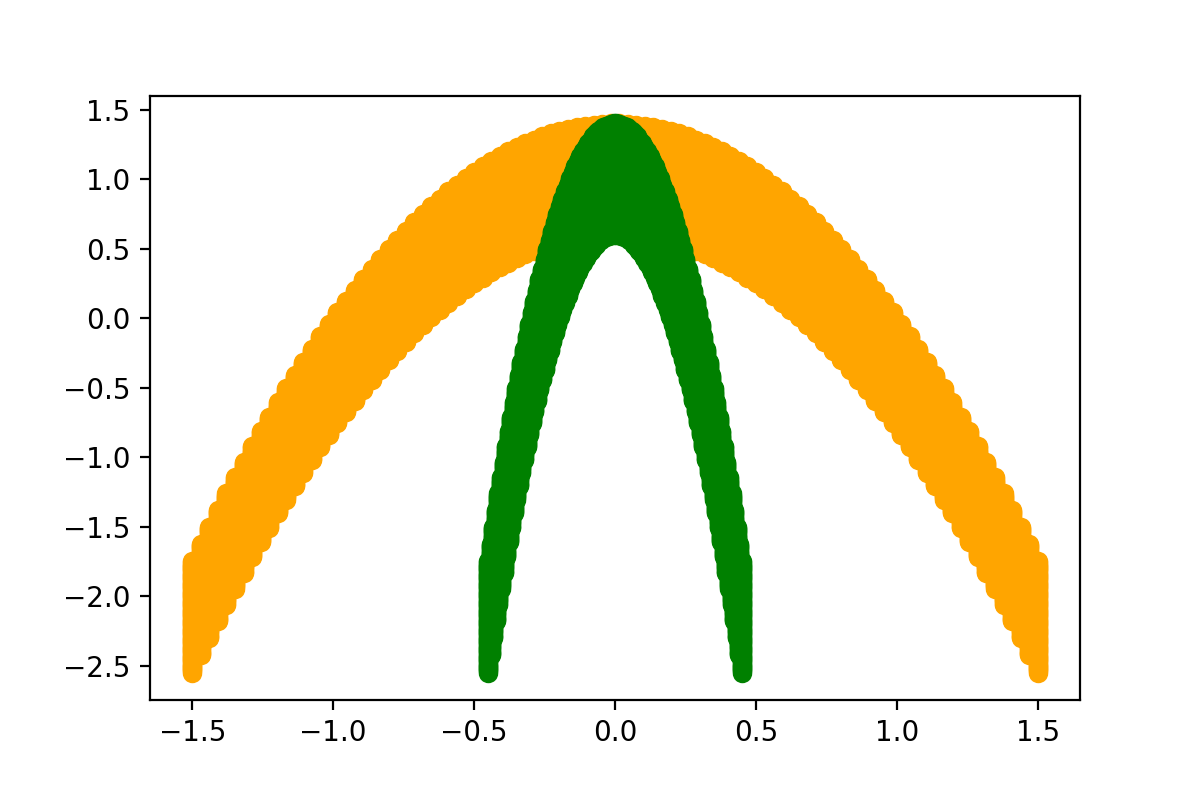
\includegraphics[width=0.3\textwidth]{figures/22_step2henon.png}
    \caption{\scriptsize seconda mappa}
    \label{fig:figures-22_step1henon-png}
\end{figure}
\noindent
In conclusione abbiamo una riflessione sulla bisettrice del primo quadrante.
\[
    \begin{cases}
        \overline{\overline{\overline{x}}} = \overline{\overline{y}}\\
	\overline{\overline{\overline{y}}} = \overline{\overline{x}}
    \end{cases}
\] 
\begin{figure}[H]
    \centering
    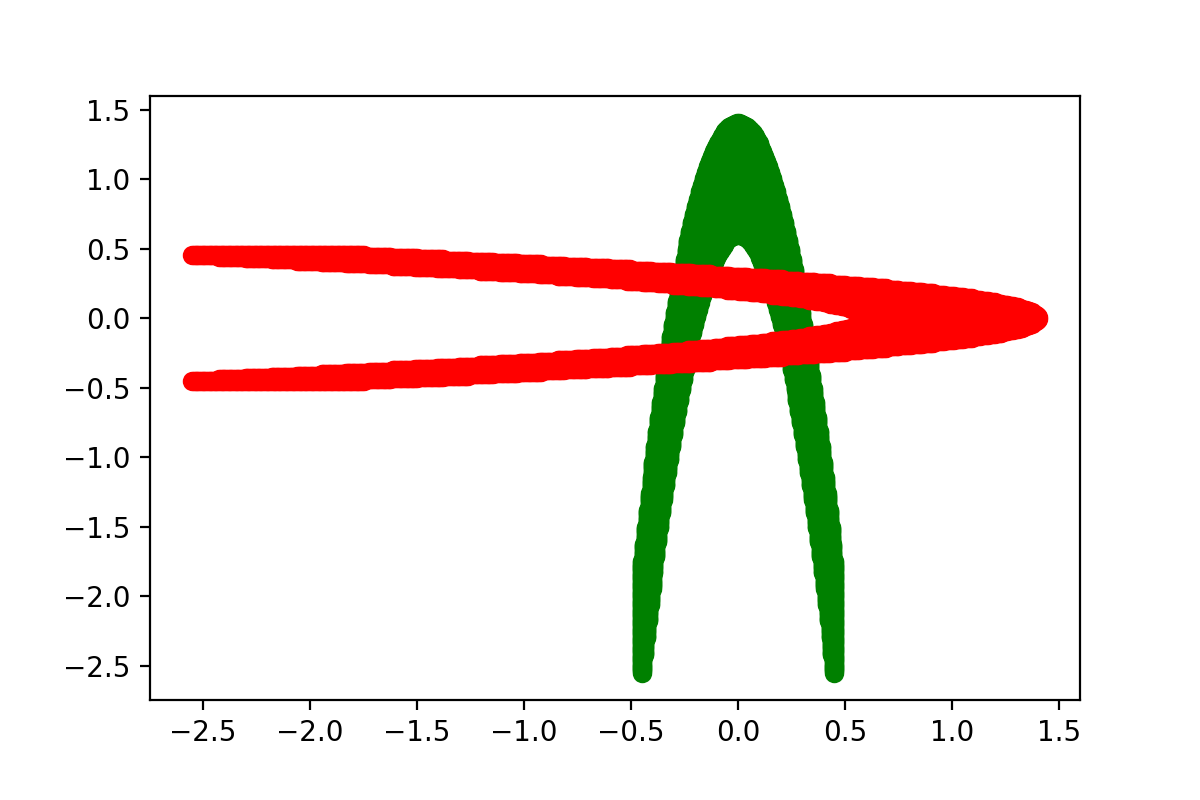
\includegraphics[width=0.3\textwidth]{figures/22_step3henon.png}
    \caption{\scriptsize Terza mappa}
    \label{fig:figures-22_step1henon-png}
\end{figure}
\noindent
\clearpage
